\documentclass[11pt,conference]{IEEEtran}

\usepackage{amsmath,amssymb,amsfonts}
\usepackage{algorithmic}
\usepackage{array,booktabs}
\usepackage{amsthm}
\usepackage{graphicx}
\usepackage{subcaption}
\usepackage{textcomp}
\usepackage{xcolor}
\usepackage[inline]{enumitem}
\usepackage{tikz}
\usetikzlibrary{matrix,calc}
\newlist{inlist}{enumerate*}{1}
\setlist[inlist]{label= (\alph*)}
\usepackage{mathpartir,semantic}
\usepackage[colorlinks]{hyperref}
\hypersetup{%
    colorlinks=true,
    linkcolor=blue,
    urlcolor=cyan,
    citecolor=blue
}
\usepackage[style=ieee]{biblatex}
\addbibresource{sources.bib}

\newcommand{\matlab}{MATLAB}
\newcommand{\mmatlab}{\textmu\matlab}
\newcommand{\colorlib}{CoLoR}
\renewcommand{\algorithmiccomment}[1]{\% #1}
\newcommand{\inputcoq}[1]{\InputIfFileExists{#1.v_tex}{}{\typeout{No file #1.v_tex.}}}
\newcommand{\var}[1]{\mathit{#1}}
\newcommand{\func}[1]{\mathsf{#1}}
\newcommand{\iname}[1]{\textsf{#1}}

\theoremstyle{plain} % default
\newtheorem{thm}{Theorem}[section]
\newtheorem{lem}[thm]{Lemma}
\newtheorem{prop}[thm]{Property}
\newtheorem*{cor}{Corollary}

\theoremstyle{definition}
\newtheorem{defn}{Definition}[section]
\newtheorem{example}{Example}[section]
\newtheorem{exercise}{Exercise}[section]
\newtheorem*{prob}{Problem}

\theoremstyle{remark}
\newtheorem*{rem}{Remark}
\newtheorem*{note}{Note}
\newtheorem{case}{Case}

\begin{document}

\title{Final paper: Towards Proving Termination of \texttt{zelda-mosaic} Algorithms under Conditions on the Input}

\author{\IEEEauthorblockN{Justin Do}
\IEEEauthorblockA{\textit{Computer Science} \\
\textit{UNC Chapel Hill}\\
Chapel Hill, USA \\
\texttt{justindo@cs.unc.edu}}
\and
\IEEEauthorblockN{D. Ben Knoble}
\IEEEauthorblockA{\textit{Computer Science} \\
\textit{UNC Chapel Hill}\\
Chapel Hill, USA \\
\texttt{david3@cs.unc.edu}}
}

\maketitle

\begin{abstract}
    We report on the development developing matrix algorithms in Coq intended to
    serve proofs about a subset of \matlab\@. Specifically, we are interested in
    a previous set of algorithms that we developed for building mosaics,
    implemented in \matlab\@. We discuss the formalization of the necessary
    matrix algorithms and the relevant \matlab\ structures in Coq~\cite{Coq}, as
    well as what remains to be done to prove the termination of the mosaic
    algorithms under appropriate to-be-determined conditions. We present details
    on the matrix development along with the key theorems for its correctness.
    We describe the challenges we faced in developing the matrix type and its
    operations, providing a glimpse at dependently-typed vectors in Coq. We also
    briefly discuss advanced automation in Coq useful for the matrix
    development.
\end{abstract}

% \begin{IEEEkeywords}
% \end{IEEEkeywords}

\section{Introduction}

We have previously developed \texttt{zelda-mosaic}~\cite{zelda_mosaic} which
includes \matlab~\cite{matlab} code to create tiled ``mosaics'' from a set of
smaller input images. In our original proposal, we set out to prove the
termination of our mosaic-generation algorithms.

In the original work, we took a series of related images (specifically, from one
of the many ``Legend of Zelda'' ({\copyright} Nintendo) games) and automatically
stitched them together to form mosaics of game-related artwork.
\figurename~\ref{F:zelda-mosaic-sample} showcases an example output. The program
is extendable and has been successfully used on several different sizes of
inputs and for applications beyond the original project.

\begin{figure*}[pht]
    \centering
    \begin{subfigure}{0.35\textwidth}
        
\includegraphics[width=\linewidth]{img/oracleofages-original.jpg}
        \caption{Original key-art}
    \end{subfigure}
    \begin{subfigure}{0.35\textwidth}
        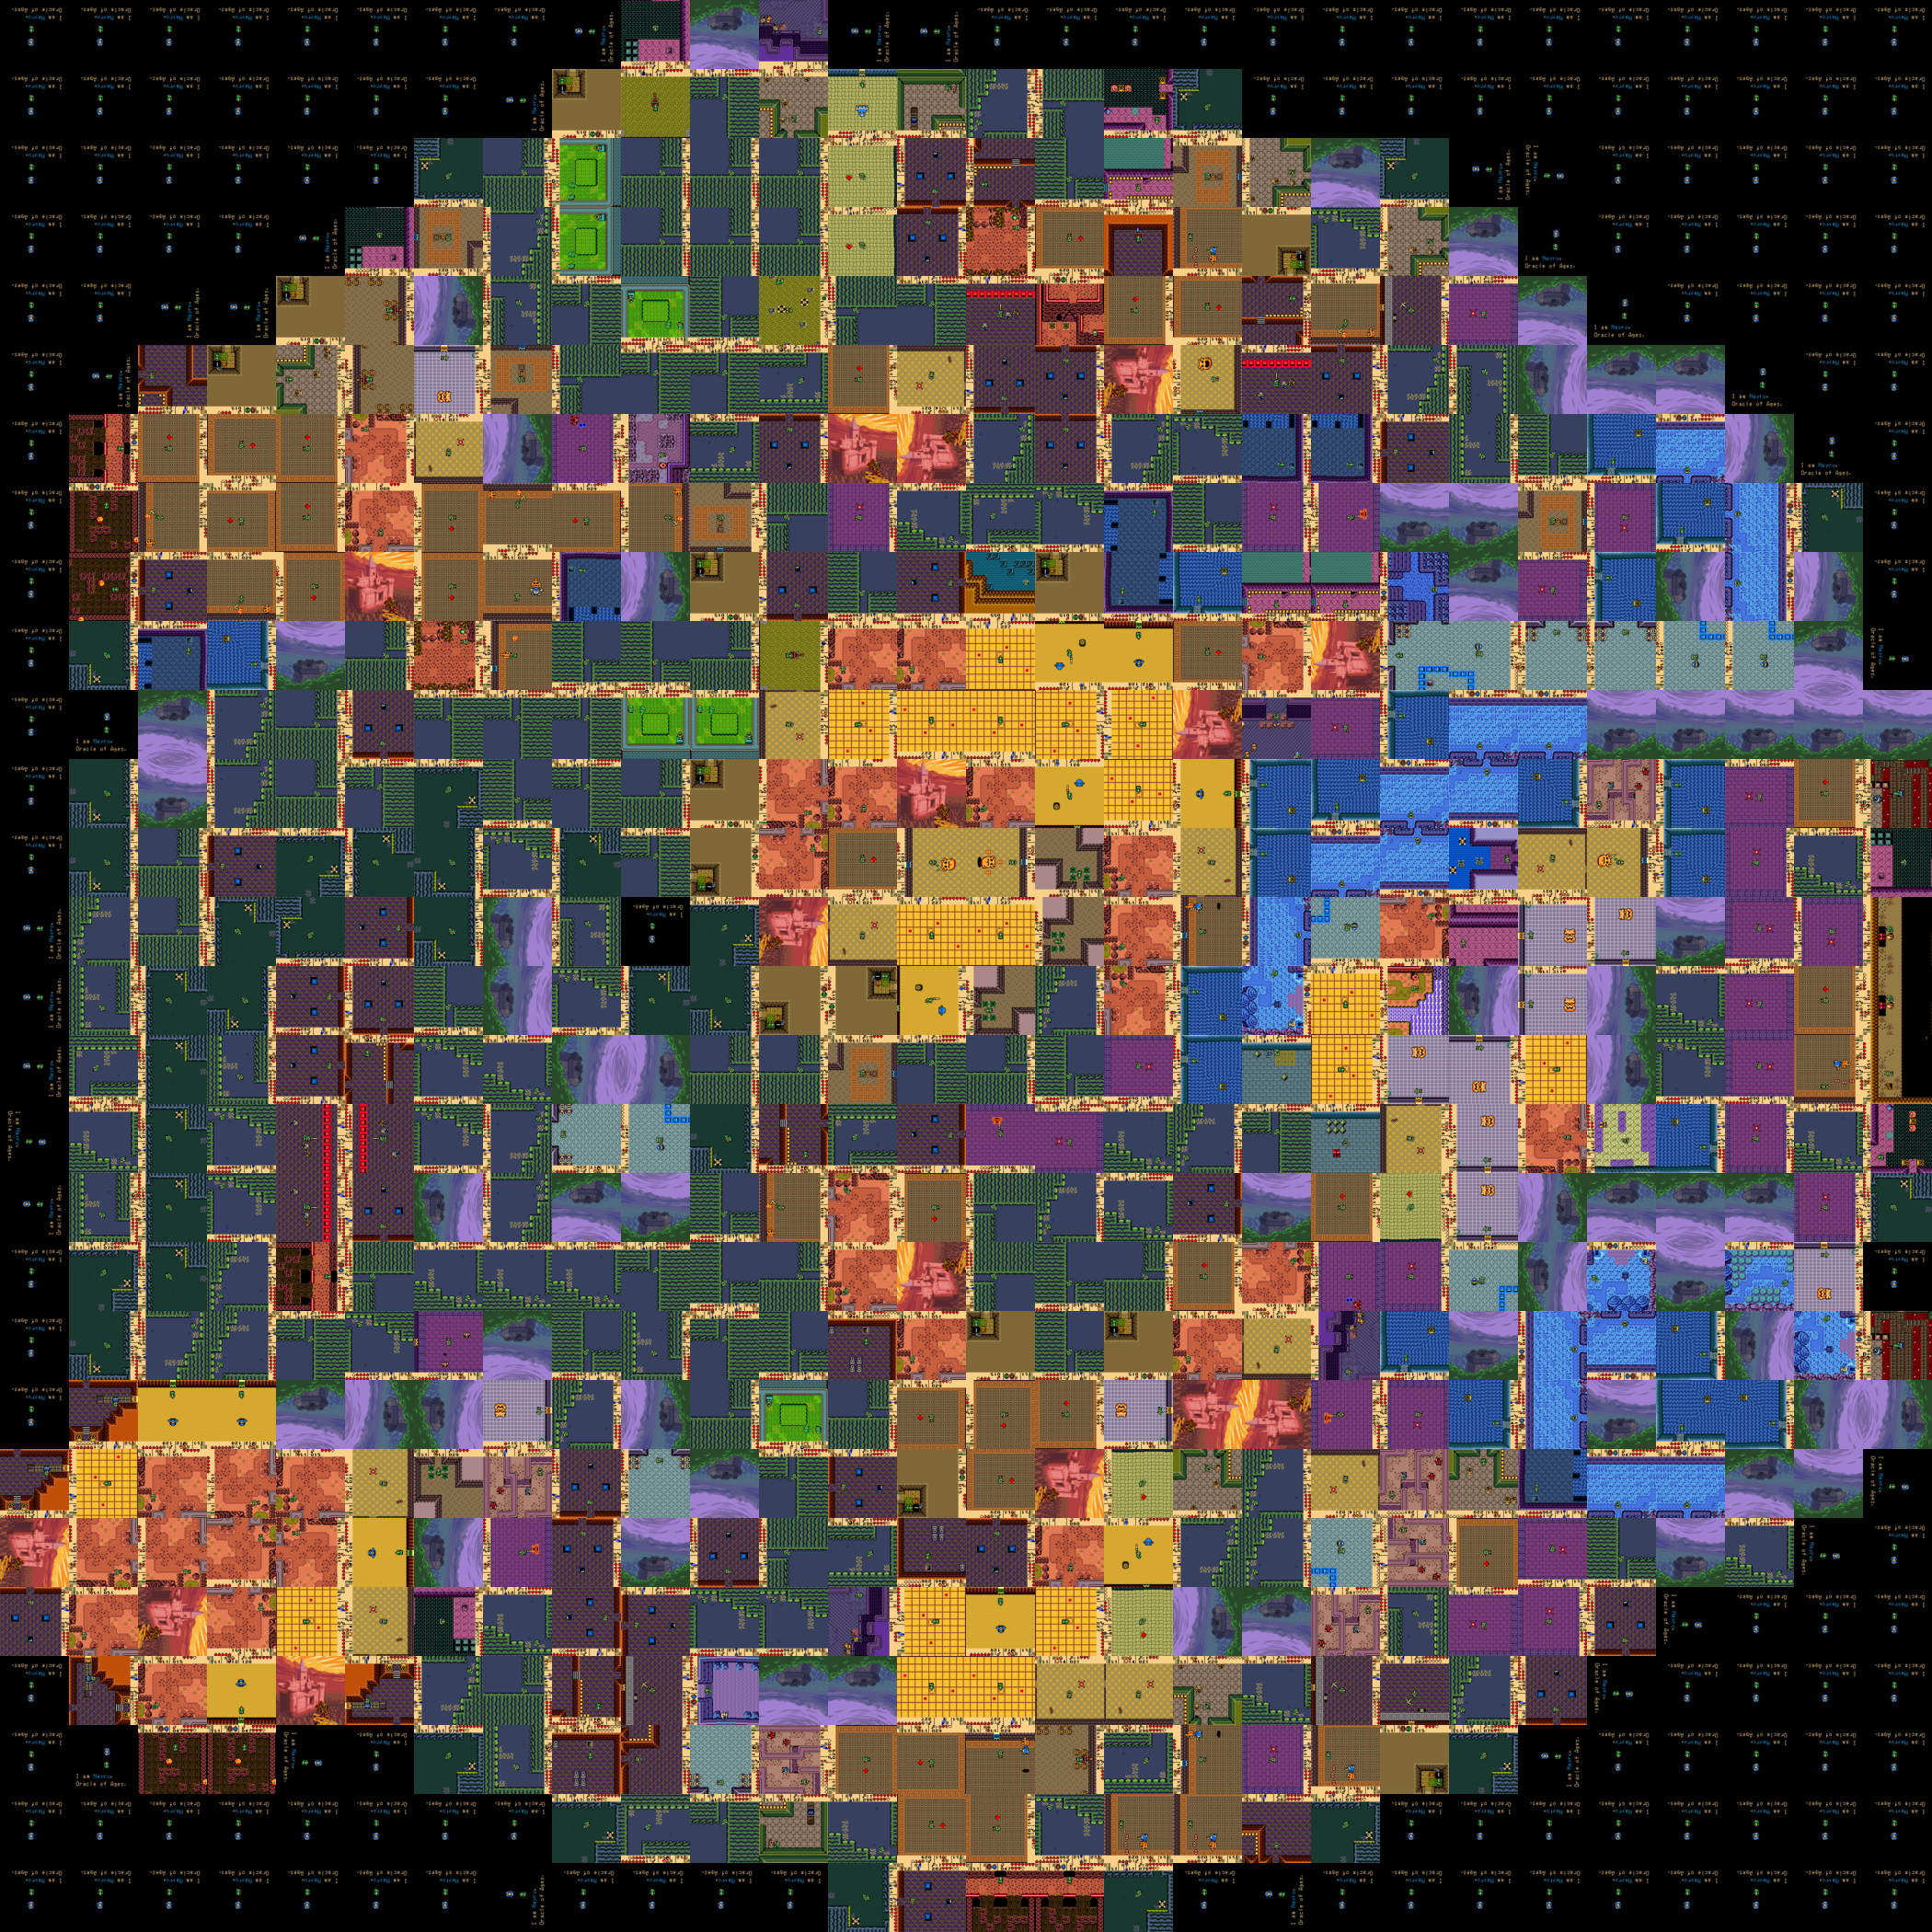
\includegraphics[width=\linewidth]{img/oracle_of_ages_v1.png}
        \caption{Version 1 Mosaic}
    \end{subfigure}
    \begin{subfigure}{0.35\textwidth}
        \includegraphics[width=\linewidth]{img/oracle_of_ages_v2.png}
        \caption{Version 2 Mosaic}
    \end{subfigure}
    \begin{subfigure}{0.35\textwidth}
        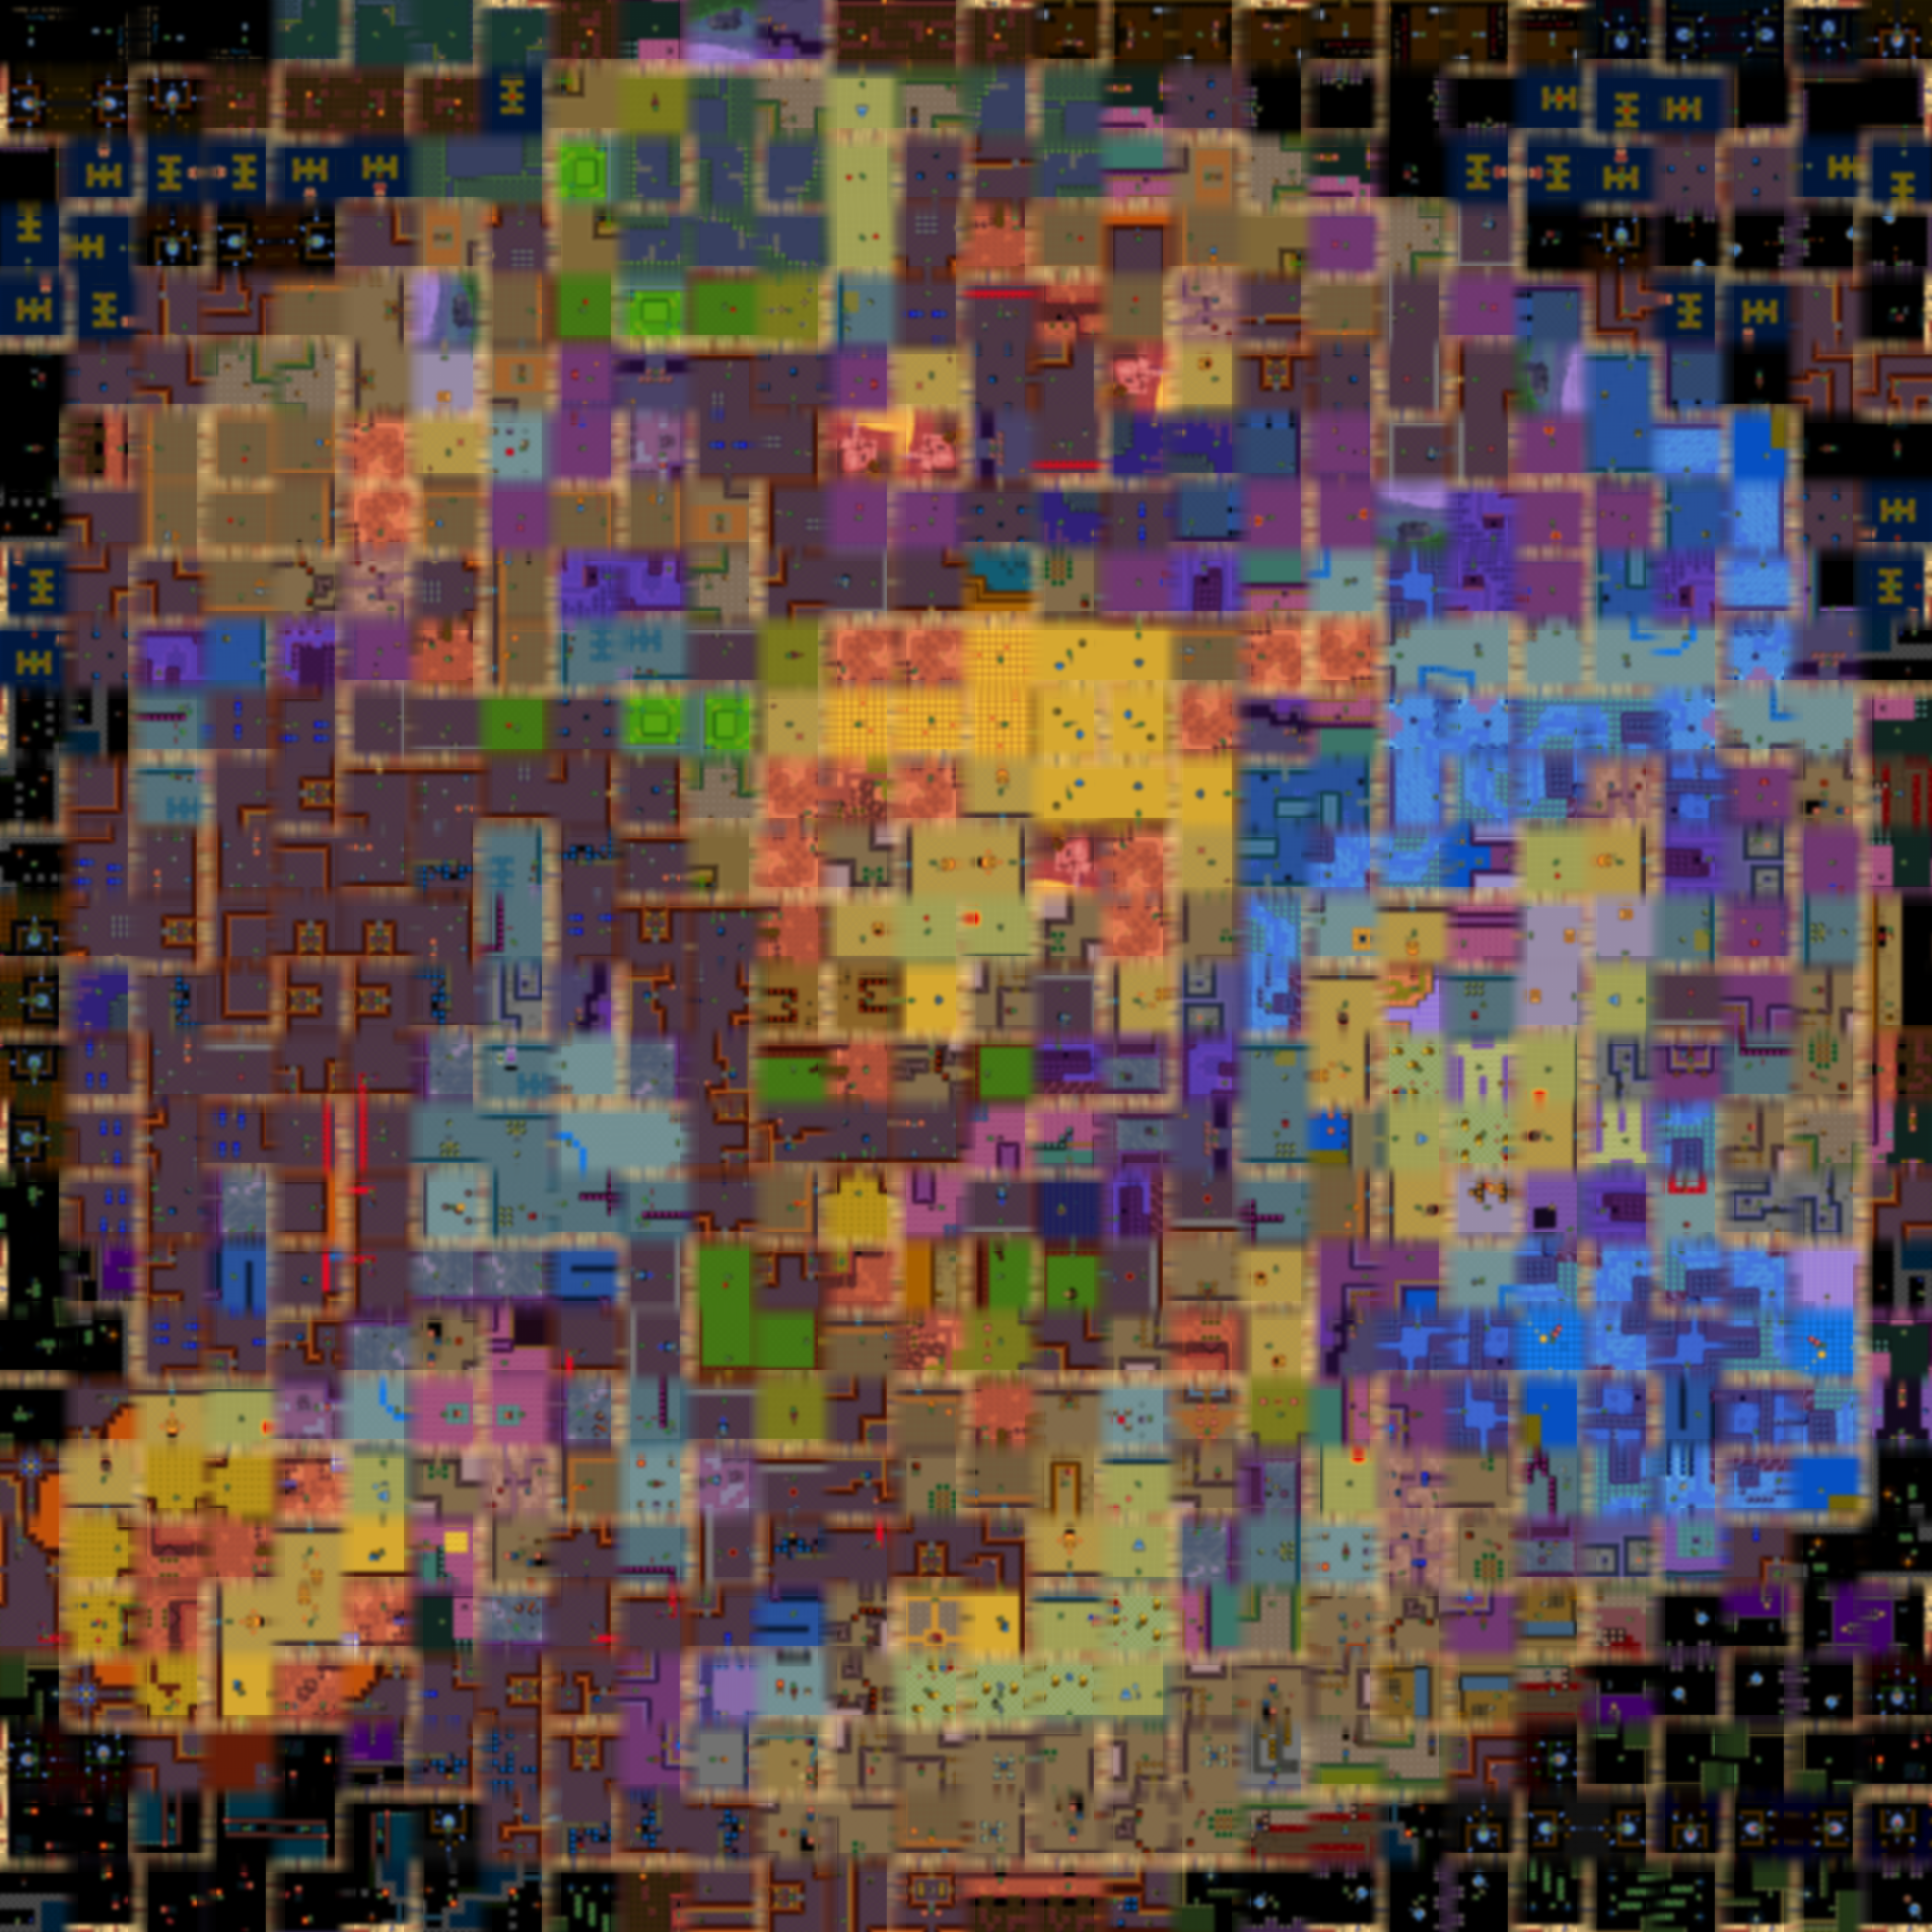
\includegraphics[width=\linewidth]{img/oracle_of_ages_v3.png}
        \caption{Version 3 Mosaic}
    \end{subfigure}
    \begin{subfigure}{0.35\textwidth}
        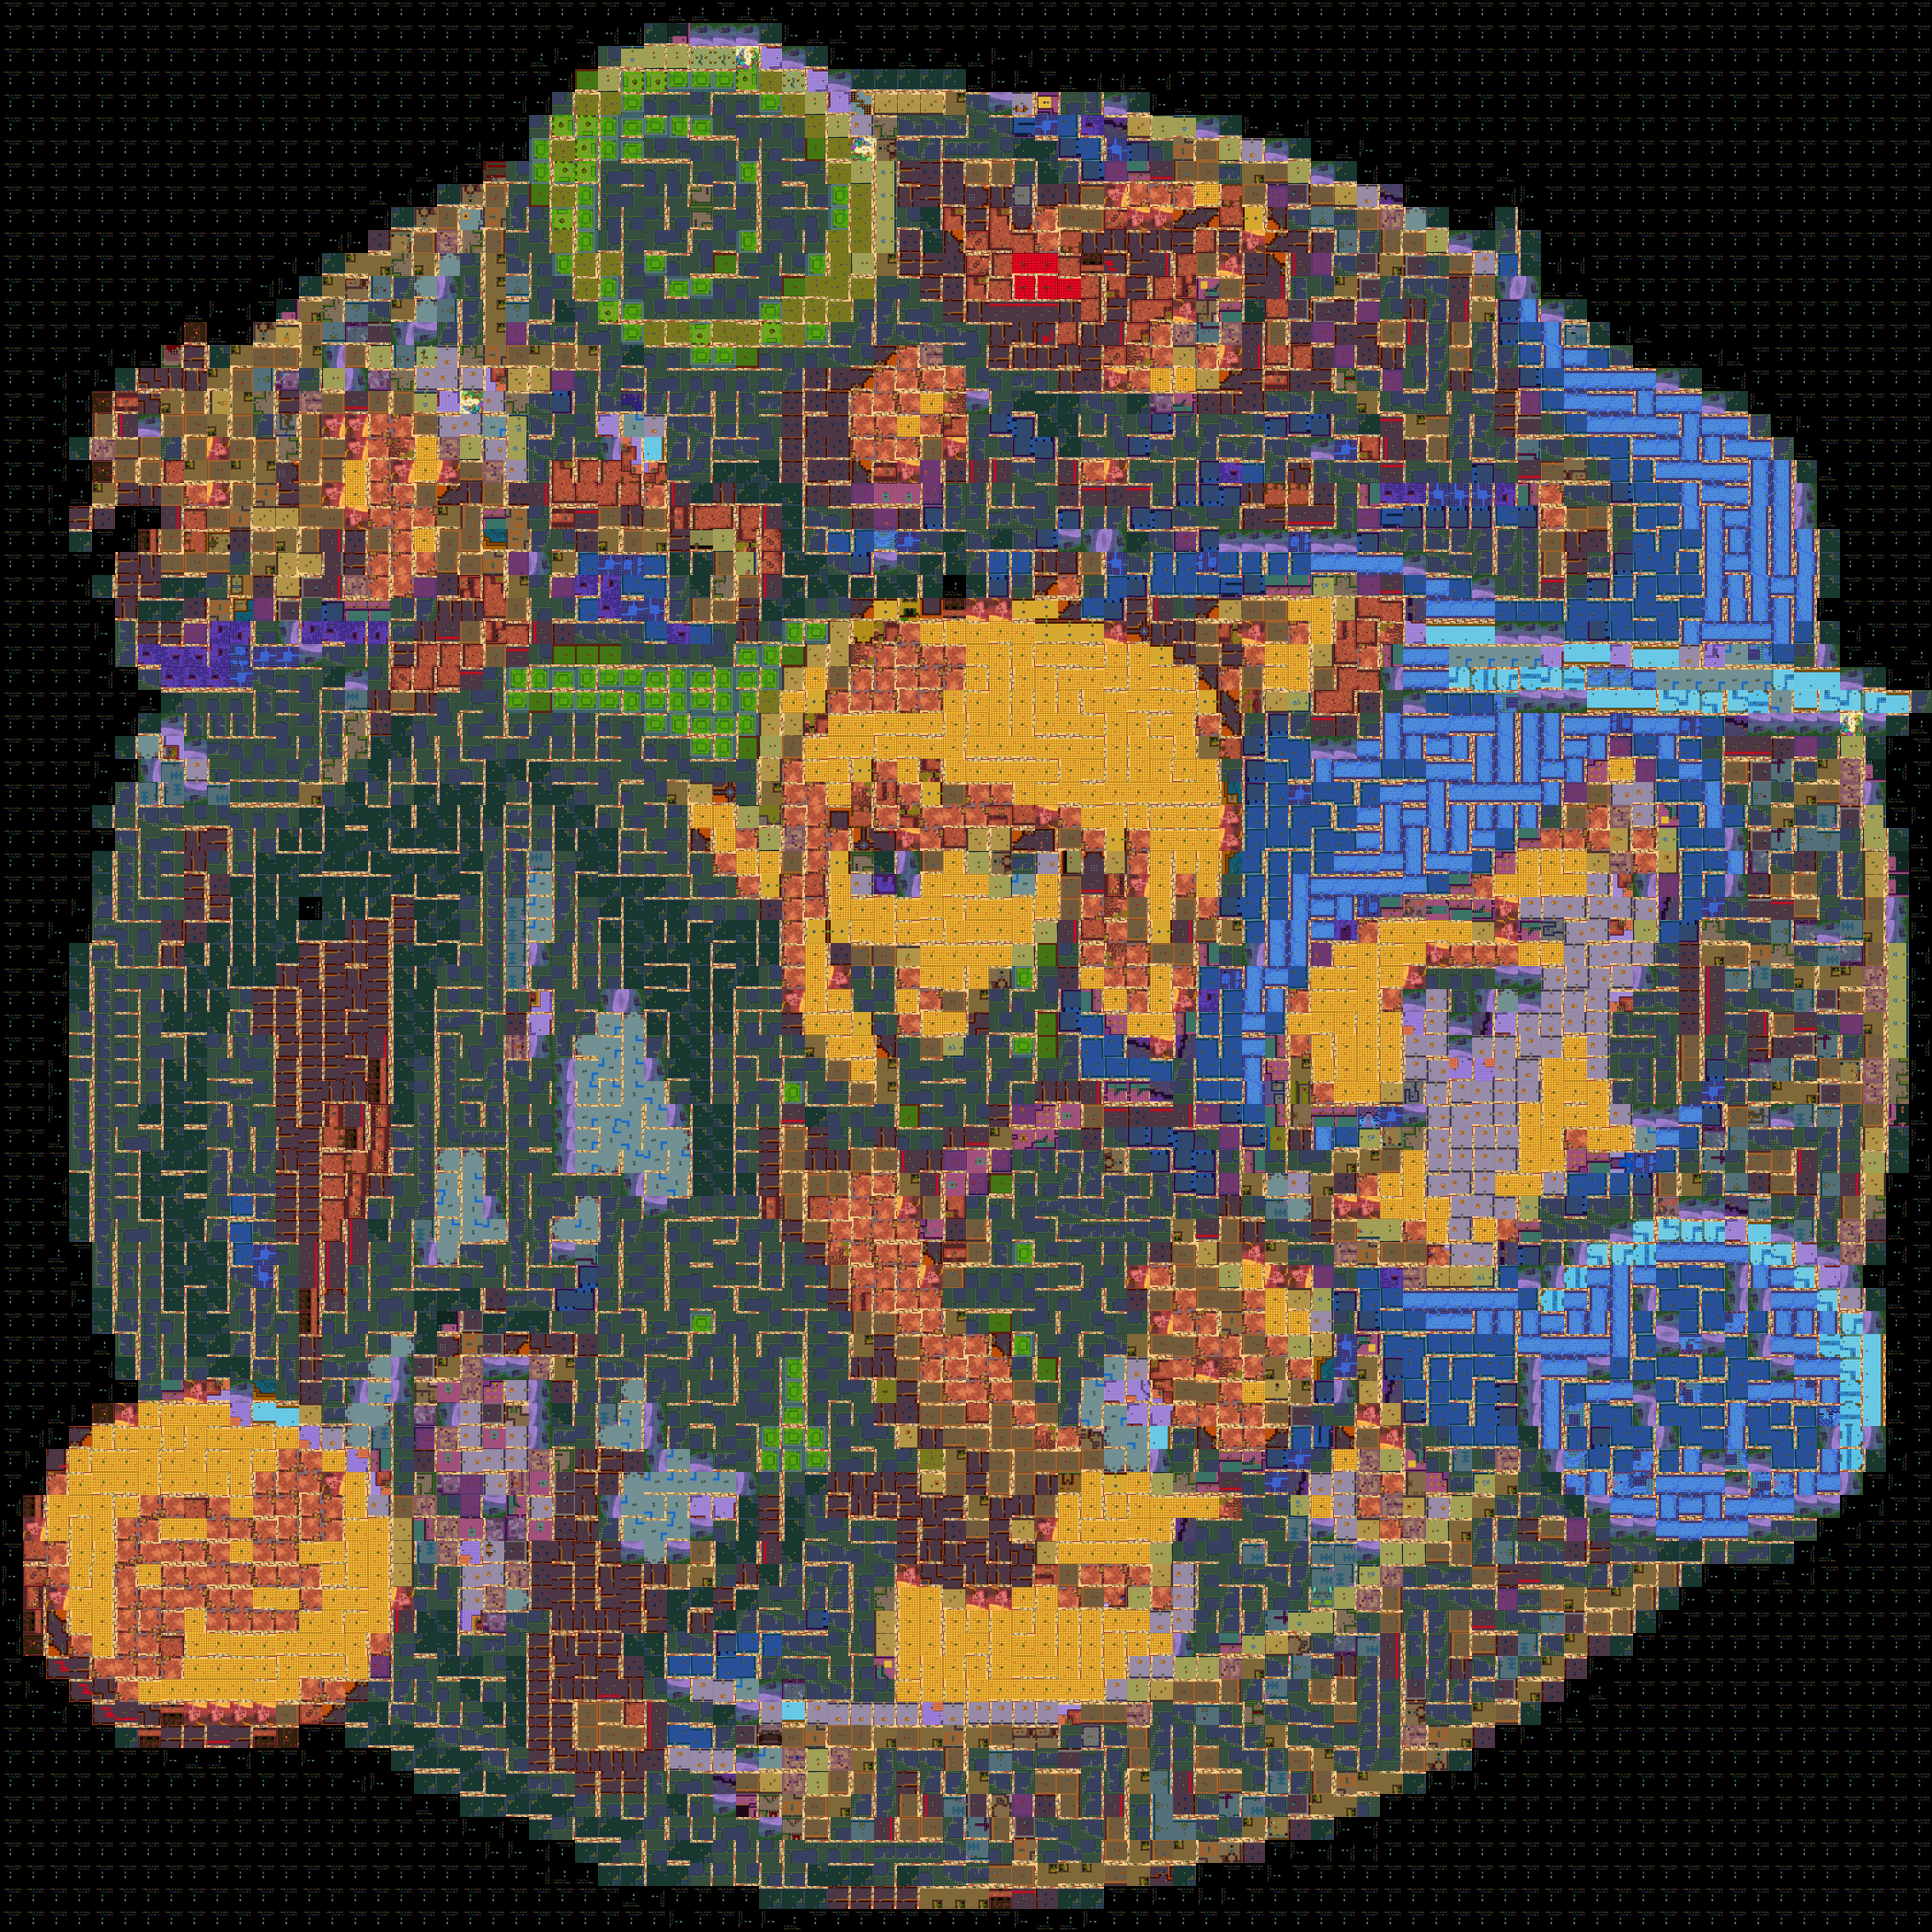
\includegraphics[width=\linewidth]{img/oracle_of_ages_v1_smaller.png}
        \caption{Version 1 Mosaic with smaller inputs}
    \end{subfigure}
    \begin{subfigure}{0.35\textwidth}
        \includegraphics[width=\linewidth]{img/oracle_of_ages_v3_smaller.png}
        \caption{Version 3 Mosaic with smaller inputs}
    \end{subfigure}
    \caption{\texttt{zelda-mosaic} sample}\label{F:zelda-mosaic-sample}
\end{figure*}

We iteratively developed three versions after our initial proof-of-concept. Each
version refines the algorithm of the previous version (for details, the
pseudocode for each algorithm may be found in
\figurename{s}~\ref{alg:v1},~\ref{alg:v2}, and~\ref{alg:v3}). We also further
refined mosaic quality by stitching smaller images, at a performance cost. The
original presentation is publicly available~\cite{zelda_mosaic_pres}, as is a
separate video-recording~\cite{zelda_mosaic_vid}.

\begin{figure}[htp]
    \textbf{Input}: image \(key\_art\), images \(thumbnails\), integer \(size\) \\
    \textbf{Output}: image \(tiles\)
    \begin{algorithmic}
        \STATE{\(tiles \gets \textrm{MAT2TILES}(key\_art, size, size)\)}
        \FOR{\(tile \in tiles\)}
            \FOR{\(thumbnail, i \in thumbnails, [1..|thumbnails| ]\)}
                \STATE{\(mses_i \gets \textrm{immse}(tile, thumbnail)\)}
            \ENDFOR
            \STATE{\(best\_indices \gets \textrm{find} (mses = \min mses)\)}
            \STATE{\(best\_index \gets best\_indices_0\)}
            \STATE{\(tile \gets thumbnails_{best\_index}\)}
        \ENDFOR
    \RETURN{\(tiles\)}
    \end{algorithmic}
    \caption{Algorithm: Version 1}\label{alg:v1}
\end{figure}

\begin{figure}[htp]
    \textbf{Input}: image \(key\_art\), images \(thumbnails\), integer \(size\) \\
    \textbf{Output}: image \(tiles\)
    \begin{algorithmic}
        \STATE{\(tiles \gets \textrm{MAT2TILES}(key\_art, size, size)\)}
        \STATE{\(used \gets \emptyset\)}
        \STATE{\(threshold \gets 1\)}
        \IF{\(|thumbnails| < |tiles|\)}
            \STATE{\(threshold \gets \lceil{|tiles| / |thumbnails|}\rceil\)}
        \ENDIF
        \FOR{\(tile \in tiles\)}
            \FOR{\(thumbnail, i \in thumbnails, [1..|thumbnails| ]\)}
                \STATE{\(mses_i \gets \textrm{immse}(tile, thumbnail)\)}
            \ENDFOR
            \STATE{\(best\_indices \gets \textrm{find} (mses = \min mses)\)}
            \STATE{\(best\_index \gets best\_indices_0\)}
            \WHILE{\(used_{best\_index} \ge threshold\)}
                \STATE{\(mses_{best\_index} \gets \infty\)}
                \STATE{\(best\_indices \gets \textrm{find} (mses = \min mses)\)}
                \STATE{\(best\_index \gets best\_indices_0\)}
            \ENDWHILE
            \STATE{increment \(used_{best\_index}\)}
            \STATE{\(tile \gets thumbnails_{best\_index}\)}
        \ENDFOR
        \RETURN{\(tiles\)}
    \end{algorithmic}
    \caption{Algorithm: Version 2}\label{alg:v2}
\end{figure}

\begin{figure}[htp]
    \textbf{Input}: image \(key\_art\), images \(thumbnails\), integer \(size\) \\
    \textbf{Output}: image \(tiles\)
    \begin{algorithmic}
        \STATE{}\COMMENT{Repeat Version 2}
        \STATE{\(tiles \gets \textrm{Version2}(key\_art, thumbnails, size)\)}
        \STATE{\(tiles \gets \textrm{imgaussfilt}(tiles)\)}
        \STATE{\(strip\_size \gets \lfloor{size / 8}\rfloor\)}
        \STATE{}\COMMENT{Blur by averaging}
        \FOR{horizontal \(strip \in tiles\)}
            \STATE{\(strip \gets \textrm{mean}({strip})\)}
        \ENDFOR
        \FOR{vertical \(strip \in tiles\)}
            \STATE{\(strip \gets \textrm{mean}({strip})\)}
        \ENDFOR
        \RETURN{\(tiles\)}
    \end{algorithmic}
    \caption{Algorithm: Version 3}\label{alg:v3}
\end{figure}

Our original goal was to examine these algorithms as implemented in the \matlab\
source and prove, if possible, their termination given well-conditioned input.
Thus we embarked on developing a Coq model of the mosaic algorithms in order to
write proofs about them. As we will explain, we did not complete this
objective---instead, we made progress on the core of the problem: defining
matrices and their operations. To that extent, we will gloss over the finer
details of \matlab\ where possible and focus specifically on the relevant matrix
operations.

In the subsequent sections, we cover related work (\S~\ref{S:related_work}),
describe the problem we tackled (\S~\ref{S:problem_desc}), our approach to
designing a solution (\S~\ref{S:design}), and our results (\S~\ref{S:results}).

\section{Related Work}\label{S:related_work}

Because we are proving something about code that we have written ourselves,
there is not a vast body of literature specific to our algorithms from which we
can draw. There are however a number of related issues exposed by our code,
which we will discuss here. In particular, the following are of interest and
have been written about:

\begin{itemize}
    \item The correctness of \matlab's \textit{cell array} data structure and
        its representation in Coq;
    \item The correctness of \matlab's built-in numerical functions and matrix
        operations; and
    \item Proving termination of a particular program based on the inputs of the
        program.
\end{itemize}

We are not the first group to demonstrate interest in proving properties about
matrix representations. In the early days of Coq, a
paper~\cite{magaud:hal-00955444} was published discussing the implementation of
square matrices in Coq, as well as proofs involving basic operations such as
addition and multiplication. This paper references \textit{Linear
Algebra}~\cite{lin_alg}, a Coq library written by a colleague which formalizes a
well-known linear algebra text~\cite{linear_algebra} and supports matrices with
a differing number of rows and columns. These implementations are specific to
two-dimesional matrices, as far as we can tell, and are thus inadequate for the
manipulation of higher dimensions in our algorithms.

\matlab\ is a closed-source piece of software, and little has been published about
its correctness. In the official \matlab\ forum, users have demonstrated interest
in verifying the correctness of \matlab\ algorithms~\cite{duenisch_2013} and the
\matlab\ staff reassure users that the algorithms have gone through rigorous
testing, but this assurance does not carry the same weight as a formal
verification. Indeed, as we have learned, these techniques fall on separate
parts of a correctness spectrum, with testing demonstrating correctness less
reliably than formal methods. The lack of related work in the \matlab\ domain
served as further motivation to obtain results about the correctness of the subset
of \matlab\ features used in our code.

Program termination is a topic of wide interest in the computing community, as
it has both practical and of theoretical relevance given the famous halting
problem. \citeauthor{Cook_2011}~\cite{Cook_2011} argue in their article that
computer scientists are often hesitant to make claims about the termination of a
particular program, but that it is often achievable. Their work draws from the
field of compilers and makes the argument that one can prove the termination of
a program given certain inputs, provided that there is sufficient analysis of
the relation between the inputs and the possible paths that may be taken during
execution\footnote{In many contexts, this involves things like symbolic
execution (cf. Rosette~\cite{Rosette}).}. Many of the ideas in this work are
formalized by \citeauthor{BLANQUI_2011} in the \colorlib\ library for Coq,
which is used primarily for proofs involving rewriting code and program
termination~\cite{BLANQUI_2011}.

\section{Problem Description}\label{S:problem_desc}

Many non-trivial programs make use of arrays, and our \texttt{zelda-mosaic}
program is no different. Because our goal was to prove the termination of the
program when given a well-formed input and the core data structure modified
throughout the program was an image (represented as an array), it is helpful to
first describe the array operations used and the invariants of an array that
contribute to the \emph{well-formed} property.

\subsection{Array Usage}

\matlab's support for multi-dimensional arrays makes it amenable to
image-processing tasks such as ours. The algorithms we wrote are described at
high-level in pseudocode in \figurename{s}~\ref{alg:v1},~\ref{alg:v2},
and~\ref{alg:v3}, but here we explain them in layman's terms to help motivate
some features of our proof.

As described in our pseudocode, the inputs to our program were a piece of
\emph{key art} to be recomposed with \emph{thumbnails} of a certain \emph{size},
which is the width and height of the square thumbnails. The original
representation of the key art in \matlab\ is a two-dimensional array (with
indices corresponding to a particular pixel's row and column) containing an
additional array of three values---one each for the red, green, and blue color
channels. In total, the array has three dimensions. We then divide this image
into \emph{chunks}, where each chunk will be replaced by a
thumbnail in the final product. For key art of dimensions $m
\times n$ (with $m$ corresponding to rows and $n$ corresponding to columns), each
image will be divided into $(m / \var{size}) \times (n / \var{size})$ chunks, which
will each be replaced by a thumbnail as appropriate. These chunks,
each of size $\var{size} \times \var{size}$, are then stored in a two-dimensional array,
with each chunk retaining its original placement in the key art.
As a result we now have a five-dimensional array, and in order to access a
particular value from a color channel, we need the following values:

\begin{itemize}
\item the \emph{chunk row} it is in
\item the \emph{chunk column} it is in
\item the \emph{x offset} of the pixel into its chunk
\item the \emph{y offset} of the pixel into its chunk
\item the \emph{color channel} desired out of red, green, and blue
\end{itemize}

Thus, once a piece of key art is successfully divided into chunks, the image is
effectively represented as an array whose dimensions correspond to the above
values. The chunks are iterated through in row-major order, gradually being
replaced in-place by thumbnails. Consequently, the state of our core array
maintains some matrix-like properties that are supported by \matlab\ arrays,
but not particular to \matlab\ in general:

\begin{itemize}
    \item The shape of a matrix \(M\) can be described by a list of \(d\)
        dimensions, where each dimension's value \(v_i\) refers to the number of
        elements held along that dimension. For example, an array with
        dimensions \(3 \times 4 \times 2\) contains 3 arrays, each of which
        contains 4 arrays of 2 elements. The dimensions list contains \(v_1 =
        3\), \(v_2 = 4\), and \(v_3 = 2\).
    \item Once the shape of \(M\) is defined and all of the elements have been
        populated, the shape will not change and all of the elements will remain
        populated. For example, the aforementioned \(3 \times 4 \times 2\) array
        must always contain 3 arrays, each of which contains 4 arrays of 2
        elements.
    \item Each \(i\)-the dimension from \(1\) to \(d-1\) must contain \(v_i\)
        elements, each of which is an array of length \(v_{i+1}\); in other
        words, the length of each element in a particular dimension must be
        identical to one another.
\end{itemize}

In summary, these properties describe the notion of a ``well-formed'' matrix
that ensures that the size \(v_i\) of each dimension remains fixed and that all
elements in a particular dimension \(i\) have the same length as one another.
This property is generally true of matrices, hence the references to both an
``arrays'' and ``matrices'' in this section. Unless otherwise noted, ``array''
refers to the generic \matlab\ object and ``matrix'' refers to an ``array'' with
these properties when discussed in the scope of this paper.

\subsection{Operations}

\matlab\ supports a number of operations that can be used to manipulate arrays,
but only a subset are used in our program. To illustrate the operations used, we
begin with the following visualization of a three-dimensional array \(E\) with
dimensions \(3 \times 4 \times 2\) and discuss how it is used in \matlab.

% Code adapted from: https://tex.stackexchange.com/questions/300109/simple-visualization-of-3d-matrix

\begin{center}
    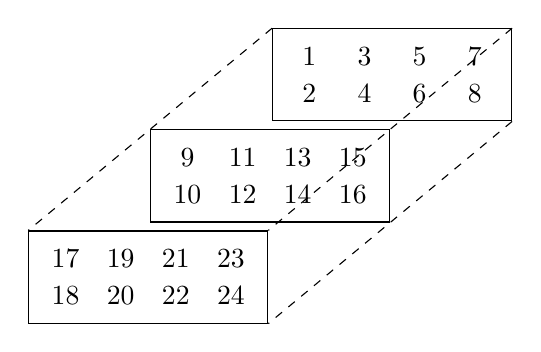
\begin{tikzpicture}[every node/.style={anchor=north east,fill=white, minimum width=.7cm}]
        \matrix (mA) [draw,matrix of math nodes]
        {
            1 & 3 & 5 & 7 \\
            2 & 4 & 6 & 8 \\
        };

        \matrix (mB) [draw,matrix of math nodes] at ($(mA.south west)-(-1.5, .1)$)
        {
            9 & 11 & 13 & 15 \\
            10 & 12 & 14 & 16 \\
        };

        \matrix (mC) [draw,matrix of math nodes] at ($(mB.south west)-(-1.5, .1)$)
        {
            17 & 19 & 21 & 23 \\
            18 & 20 & 22 & 24 \\
        };

        \draw[dashed](mA.north east)--(mC.north east);
        \draw[dashed](mA.north west)--(mC.north west);
        \draw[dashed](mA.south east)--(mC.south east);
    \end{tikzpicture}
\end{center}

\subsubsection{Element Access}

For the matrix \(E\), each element would be indexed according to the following
mapping. Under this scheme, for example, the element \(8\) in \(E\) would
have the index \((1, 4, 2)\). This indexing scheme is the general pattern used to
access one particular element out of a multi-dimensional array. Note that arrays
in \matlab\ have indices starting at 1. The indexing scheme is demonstrated
below.

\begin{center}
    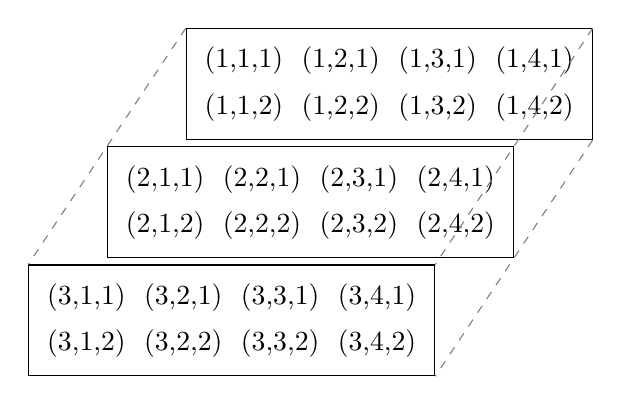
\begin{tikzpicture}
        \def\xs{1} %shift in x direction
        \def\ys{1.5} %shift in y direction
        \def\nm{3} % number of 2d matrices in the 3d matrix
        \foreach \x in {1,2,...,\nm}
        {
            \matrix [draw, % for the rectangle border
            fill=white, % so that it is not transparent
            ampersand replacement=\&] %see explanation
            (mm\x)%give the matrix a name
            at(-\x * \xs, -\x * \ys) %shift the matrix
            {
                \node {(\x,1,1)}; \& \node {(\x,2,1)}; \& \node {(\x,3,1)}; \& \node {(\x,4,1)};\\
                \node {(\x,1,2)}; \& \node {(\x,2,2)}; \& \node {(\x,3,2)}; \& \node {(\x,4,2)};\\
            };
        }

        \draw [dashed,gray](mm1.north west) -- (mm\nm.north west);
        \draw [dashed,gray](mm1.north east) -- (mm\nm.north east);
        \draw [dashed,gray](mm1.south east) -- (mm\nm.south east);
    \end{tikzpicture}
\end{center}


\subsubsection{Linearized Indexing}\label{S:linearized_indexing}

Note that in \(E\), elements are ordered in ascending order with respect to
their indexing. First, sub-array \((1)\) is populated, and \((1, 1)\) is the
first array within it, so it is filled with elements \(1\) and \(2\). Array
\((1, 2)\) is then populated by elements \(3\) and \(4\). After all four of
\(E\)'s sub-arrays have been populated, sub-array \((2)\) is populated, and so
on until the array is full.

Given the numbering scheme in \(E\), one can imagine a ``flattened'' version of
\(E\) that is an one-dimensional array containing all of \(E\)'s elements;
simply put, an array containing the elements \(1\) to \(24\) in numerical
order. \matlab\ actually allows arrays of arbitrarily many dimensions to be
logically flattened during accesses so that elements can be accessed with one
index, like in a one-dimensional array. We found this property to be somewhat
interesting and challenging to model, and we refer to the flattening of a matrix
as ``linearization.''

The process of linearizing a matrix is perhaps better explained with a
two-dimensional example. Imagine a general two-dimensional \(3 \times 4\) matrix,
such as the one below, where:
\begin{equation*}
    \begin{bmatrix}
        a & b & c & d \\
        e & f & g & h \\
        i & j & k & l
    \end{bmatrix}
\end{equation*}
To linearize the matrix, we label each value with an increasing index from the
top-left, left-to-right, top-to-bottom. For example:
\begin{equation*}
    \begin{bmatrix}
        a_1 & b_2 & c_3 & d_4 \\
        e_5 & f_6 & g_7 & h_8 \\
        i_9 & j_{10} & k_{11} & l_{12}
    \end{bmatrix}
\end{equation*}
Finally, we create a vector, a one-dimensional matrix, by reading the elements
off in order:
\setcounter{MaxMatrixCols}{20}
\begin{equation*}
    \begin{bmatrix}
        a & b & c & d & e & f & g & h & i & j & k & l
    \end{bmatrix}
\end{equation*}
This process generalizes to higher dimensions. The length of the resulting
vector is always the product of the sizes of the dimensions. To see this, note
that this product counts the number of elements in the matrix and that the
linearized matrix has the same number of elements in a single dimension.

Under this scheme, any element in a matrix can be accessed via its position in
the linearized version of that matrix. For example, the element \(12\) in \(E\)
can be accessed by the index \((12)\) and in the previous example, the element
\(f\) can be accessed by the index \((6)\).

\subsubsection{Ranged Indexing}\label{S:ranged_indexing}

Broadly speaking, \matlab\ supports the notion of a range of numbers specified
by a starting index and a stopping index, which includes every index between the
starting index and the stopping index (inclusive). This abstraction can be used
to access or assign elements within a sub-matrix of a particular matrix. For
example, suppose in matrix \(E\) you only cared about the first matrix in the
first dimension; the second, third, and fourth columns within the second
dimension; and the second row within the third dimension. This sub-matrix can be
specified by the index \((1, 2:4, 2)\) and would be the matrix

\begin{equation*}
    \begin{bmatrix}
        4 & 6 & 8
    \end{bmatrix}.
\end{equation*}

Suppose that you wanted to get the second, third, and fourth columns within the
second dimension and the second row within the third dimension for \emph{all
three} of the outer-most dimension of \(E\) but did not know \textit{a priori}
how many elements it had. \matlab\ supports an ``inclusive range'' operator,
represented by a colon \texttt{:}. This operator represents the range
encompassing all values in a particular dimension. The sub-matrix described here
would be specified by the index $(:, 2:4, 2)$ and represents the following
matrix:

\begin{center}
    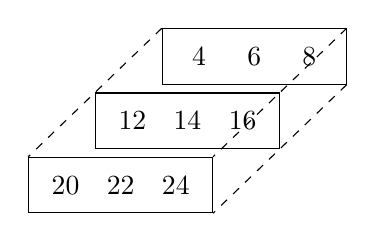
\begin{tikzpicture}[every node/.style={anchor=north east,fill=white, minimum width=.7cm}]
        \matrix (mA) [draw,matrix of math nodes]
        {
            4 & 6 & 8 \\
        };

        \matrix (mB) [draw,matrix of math nodes] at ($(mA.south west)-(-1.5, .1)$)
        {
            12 & 14 & 16 \\
        };

        \matrix (mC) [draw,matrix of math nodes] at ($(mB.south west)-(-1.5, .1)$)
        {
            20 & 22 & 24 \\
        };

        \draw[dashed](mA.north east)--(mC.north east);
        \draw[dashed](mA.north west)--(mC.north west);
        \draw[dashed](mA.south east)--(mC.south east);
    \end{tikzpicture}
\end{center}

\subsubsection{Matrix Operations}\label{S:matrix_operations}

Details about \matlab\ arrays pertaining to indexing are perhaps some of their
most interesting features, but we also use some typical matrix operators in our
program. Generally speaking, matrix operators can be generalized to any number
of dimensions, as long as the dimensions of the arrays agree for the operation
in question. There are two broad classes of matrix operators that we make use
of:

\begin{description}
    \item[Element-wise] For two matrices of the same dimensionality, the
        operator is applied on each of the two elements containing the same
        index in the two matrices.
    \item[All Elements] For an array and a scalar, the operation and scalar
        (\textit{e.g.}, add 1) is applied to every element in the matrix.
\end{description}

\subsection{Modeling the Problem}

Aside from the core matrix operations, we anticipated that we would need to
model the state of our program at all points of execution since our goal was to
prove termination. To this end, we would need to identify all of the syntax that
we use in our program and specify their associated semantics. The upshot of
modeling our program in this way would be the ability to remains to prove its
termination of our given that certain preconditions hold.

Hoare logic~\cite{Hoare_1969} is a type of logic that is often used to solve
problems of this class. Partial Hoare logic is a weak statement about programs;
namely, given preconditions \(P\) and postconditions \(Q\) and a program \(C\),
the Hoare triple \(\{P\}C\{Q\}\) asserts that \emph{if} \(C\) terminates, then
the pre-conditions imply the post-conditions. Total Hoare logic, by contrast, is
a stronger version of this claim: \(C\) is asserted to terminate. Thus a proof
in total Hoare logic necessitates a proof that \(C\) terminates; the inference
rules are accordingly adjusted. The primary adjustment is to the rule for while
loops, which are guaranteed to terminate by relation to a decreasing sequence
(with respect to a well-founded order).

When we started this project, we had in mind that the preconditions would be
statements about the program's inputs; for example, ``the length and width of
key art are always multiples of the thumbnails' size.'' Ultimately, we did not
get far enough in modeling our program to devise a set of pre-conditions, but
the point remains that we needed to be able to model the control flow of our
entire program in order to do this.

\section{Design and Approach}\label{S:design}

We first set out to define the syntax and semantics of the subset of \matlab\
used in our program, making the assumption that once we finished this it would
be somewhat trivial to bind the defined syntax to behavior in Coq. Ultimately,
the majority of our effort in this project ended going towards the
implementation of our multi-dimensional matrix operations, which was made
difficult by the number of properties that our matrices uphold as well as our
desire to write generic Coq functions that would work on matrices of arbitrarily
many dimensions. We spent a while working with Coq's built-in \textsf{Vector}
type before coming to the conclusion that its dependent typing caused
difficulties in behavior specification. To this end, we ended up implementing
our own data types to describe the state of matrices in our program; this task
was unexpectedly challenging and once we began working on it, it became the only
thing we worked on for the remainder of the project.

\subsection{\mmatlab}\label{S:mmatlab}

We present a brief overview on \mmatlab, the subset of \matlab\ that we modeled in
order to prove facts about our programs.

Aside from general programming patterns for control flow, the main syntax of
relevance in our program involves array/matrix accesses and updates, arithmetic
operations, and \matlab-specific primitives such as ranges. We have identified
all of the expressions and statements we expected to use and defined them as
inductive types, shown in \figurename~\ref{fig:inductivetypeexp} and
\figurename~\ref{fig:inductivetypestmt}.

\begin{figure}[ht]
    \centering
    \begin{align*}
        \func{exp} \triangleq\;
        & |\; \func{IntLiteral} \\
        & |\; \func{FloatLiteral} \\
        & |\; \func{AddExp} \\
        & |\; \func{MultExp} \\
        & |\; \func{DivExp} \\
        & |\; \func{EqualsExp} \\
        & |\; \func{NotEqualsExp} \\
        & |\; \func{LTEqualsExp} \\
        & |\; \func{Floor} \\
        & |\; \func{VarRefExp} \\
        & |\; \func{RangeExp} \\
        & |\; \func{MatrixLiteral} \\
        & |\; \func{IndexExp} \\
        & |\; \func{SqueezeExpr} \\
        & |\; \func{SizeExpr} \\
        & |\; \func{LengthExpr} \\
        & |\; \func{ProdExpr} \\
        & |\; \func{SumExpr} \\
        & |\; \func{MinExpr} \\
        & |\; \func{MaxExpr} \\
        & |\; \func{PointWiseExpExp} \\
        & |\; \func{ZerosExp} \\
        & |\; \func{OnesExp} \\
        & |\; \func{InfExp} \\
        & |\; \func{FindExp}
    \end{align*}
    \caption{Skeleton of abstract syntax for expressions used in
    \mmatlab\@.}\label{fig:inductivetypeexp}
\end{figure}

\begin{figure}[ht]
    \centering
    \begin{align*}
        \func{statement} \triangleq\;
        & |\; \func{NoOp} \\
        & |\; \func{Error} \\
        & |\; \func{ExprS} \\
        & |\; \func{AssignS} \\
        & |\; \func{IndexedAssignS} \\
        & |\; \func{SeqS} \\
        & |\; \func{WhileS} \\
        & |\; \func{IfThenElseS} \\
    \end{align*}
    \caption{Skeleton of abstract syntax for statements used in
    \mmatlab\@.}\label{fig:inductivetypestmt}
\end{figure}

Much of the abstract syntax is relatively self-explanatory, so complete
definitions are elided here. However, we wish to draw attention to some of the
less apparent and more interesting syntax present in \mmatlab:

\begin{itemize}

    \item \textsf{AddExp}: While this is nominally a regular addition operator,
        \matlab's addition is interesting in that it has overloaded parameter
        types and expected behavior for each. The addition of two numbers is a
        number and the addition of two matrices results in element-wise
        addition, as one might expect. However, the sum of a number and a
        matrix, is a matrix with all elements incremented by the number. Similar
        behaviors hold for \textsf{MultExp} and \textsf{DivExp}.

    \item \textsf{RangeExp}: Like Python, \matlab\ has an expression where a
        starting number and stopping number may be provided, generating an
        inclusive list of all numbers between them. This is discussed in
        \S~\ref{S:ranged_indexing}.

    \item \textsf{IndexExp}: This expression pairs a variable with an indexer,
        which can be an almost arbitrary expression. \matlab\ does restrict the
        syntactic placement of certain indexing operations.

    \item \textsf{SqueezeExpr}: For multi-dimensional arrays, sometimes the size
        of a particular dimension will be 1. \texttt{squeeze} is a function that
        reduces dimensionality by discarding or ``squeezing'' these superfluous
        dimensions.

\end{itemize}

We made an effort to specify each of the statements and expressions according to
Backus-Naur form, considering the syntax of which each statement or expression
was composed and instances of overloading. Our next goal was to model the state
of our program's core matrix data structure so that we could bind syntax to
semantics. For reasons that we will soon delve into, we did not progress further
than that step, so our discussion on syntax and semantics ends here. However,
had we gotten to the point of tying it all together, it would have looked very
similar to the \textit{Simple Imperative Programs} chapter in \textit{Logical
Foundations}~\cite{Pierce:SF1}.

\subsection{Blocked by Built-ins}

Thinking that there was no need to re-invent the wheel, we began our journey in
defining matrix behavior with an exploration into a standard Coq library. Along
the way, we discovered a number of interesting implementations and proof
paradigms. Ultimately, we concluded that these would be too difficult to work
with and that we were better off developing our own implementation. Here we
discuss the structures from the Coq library that we considered using and the
limitations that led us away from them.

\subsubsection{Vector}

The natural candidate in the Coq library to use for representing
multi-dimensional matrices was the \textsf{Vector} type, which was originally
implemented in the \colorlib\ library~\cite{BLANQUI_2011} and later ported to
the Coq standard library. We thought that this would be a good abstraction since
multi-dimensional matrices can have arbitrarily many dimensions and
\textsf{Vector}s are polymorphic, allowing them to contain other
\textsf{Vector}s (provided that all contained vectors are of the same type). To
aid this discussion, the definition of Coq's \textsf{Vector} is stated below:

\begin{verbatim}
Inductive t A : nat -> Type :=
| nil : t A 0
| cons : forall (h:A) (n:nat),
           t A n -> t A (S n).
\end{verbatim}

The key thing to make note of is that \textsf{Vector} is a dependent
type~\cite{Bove2009,Thorsten_2010}; the number of elements in a \textsf{Vector}
is part of its type, written \texttt{Vector.t A n} for a vector containing \(n\)
elements of type \(A\)\footnote{The Coq programmer works with dependent types
all the time, but may not realize it: hypotheses whose types depend on
quantified variables (\textit{e.g.}, the hypothesis \(H: n \le 0\)) are
dependently typed as well.}. Since the length of a particular \textsf{Vector} is
encoded in its type, it is possible to enforce the requirement that all elements
in a particular dimension have the same length. From here, we devised a scheme
to stack \textsf{Vector}s to form, \emph{e.g.}, \texttt{Vector.t (Vector.t A m)
n} such that this we could create matrices of arbitrarily many dimensions, each
of which has a fixed number of elements. To support this, we defined a
type-constructor \textsf{matrix} taking a list of dimensions, which represents a
\textsf{Vector} of \textsf{Vector}s. It can be used as the type of an arbitrary
\(n\)-dimensional matrix containing elements of type \(A\). This definition is
as follows:

\begin{verbatim}
Fixpoint matrix
        (A: Type) (dims: list nat) :=
  match dims with
  | [] => A
  | head::tail =>
        Vector.t (matrix A tail) head
  end.

\end{verbatim}

This definition worked out nicely at first, and we were able to implement
behavior such as the linearization and element access of a matrix. Although
possible, this task was non-trivial due to the arbitrary dimensionality of our
matrices and due to the proof burden imposed on functions over dependent
types~\cite{SO_2021_1}. Additionally, the existing implementation of element
access in Coq's \textsf{Vector} type uses the unfamiliar \textsf{Fin} type, an
abstraction for carrying proofs that a particular number belongs to finite range
of numbers. In order to access an element of a \textsf{Vector}, one must supply
such a proof; for our purposes, we use \texttt{Fin.of\_nat}, which gives either
such a proof or a witness that the number is outside the range. The complexity
of using the Coq built-ins was quickly growing, and we could deal with it to a
point but soon ran into trouble while implementing ranged expressions.

\subsubsection{Out of Options}

The problem we experienced while implementing ranged expressions is complex, so
here we provide an attempt to explain the essence of the problem. The full
details are available on StackOverflow, where we asked for
assistance~\cite{SO_2021_2}. The general flavor of the problem is that when
accessing indices over a range in a matrix, it is impossible to know \textit{a
priori} the shape of the returned matrix, which in turn informs the returned
matrix's type (since it is dependently typed based on its dimensionality). This
computation can be made dynamically for valid ranges, but we run into issues
when handling degenerate cases---for instance, a range containing values that
are out of bounds or a list of indices containing the wrong number of indices
for a particular matrix. In these situations, it is desirable to not return a
matrix type at all, since the behavior is undefined and will not result in a
legitimate matrix. The crux of the problem is that with the dependent types, it
was difficult to specify what dimensions an invalid matrix should have, and the
general strategy of using \textsf{Option}'s \textsf{Some} and \textsf{None}
wrappers also did not work because it requires type specification (which is what
we were having difficulty doing in the first place). Presented with this
dilemma, we heeded the advice of a commenter on our StackOverflow post, which
was to eschew dependent types altogether and build our own implementation of
matrices. The results of doing so encompass the main body of our work, and are
described in detail in \S~\ref{S:results}.

\section{Results}\label{S:results}

In this section, we present the results of our work towards proving termination
of our mosaic algorithm. As noted, our primary accomplishment is the definition
of a workable matrix type and operations on it. This matrix type is intended to
support the operations needed to implement expression evaluation for \mmatlab, a
crucial component of implementing the language's semantics. It remains to finish
implementing expression evaluation and the necessary matrix operations, to give
operation semantics for the statements of \mmatlab, to give a total Hoare logic
for the language, and then finally to give the proofs of termination of the
algorithms found in \figurename{s}~\ref{alg:v1},~\ref{alg:v2}, and~\ref{alg:v3}.

We present, in order,
\begin{inlist}
\item the Coq definition of the polymorphic matrix type \texttt{matrix A} and
    corresponding operations;
\item key theorems and sketches of their proofs about the matrix type and its
    operations; and
\item advanced tactics, automation, and ideas for Coq proofs used in the
    development.
\end{inlist}

% TODO: update zelda_mosaic_proof version with final commit

All code may be found at the project repository~\cite{zelda_mosaic_proof}. Most
of the work in this section corresponds to the file \texttt{LibMatrix.v}.

\subsection{Defining Matrices}\label{S:matrix_defn}

First, we define the matrix type. After noting that it allows invalid matrices
to be formed, we define the well-formed property on matrices in two equivalent
ways. Finally, we give an overview of the Coq definitions of three operations on
matrices: computing their shape, linearizing, and linear indexing. We briefly
mention the beginning of our work on multi-dimensional and range-based indexing.

\subsubsection{The matrix type}

As mentioned in \S~\ref{S:design}, our original formulation of matrices as
nested dependent \texttt{Vector.t}s quickly grew in complexity. We abandoned
that approach in favor of a type that is not guaranteed to behave well, but
whose definition makes defining operations more natural~\cite{SO_2021_2}. This
approach removes the proofs that dependent types provide automatically, so we
have to give those ourselves.

The new design pairs the dimensionality of a matrix, called its \emph{shape},
with its \emph{contents}. The pairing is done via \emph{Record} types (see the
Coq manual~\cite{Coq}), which are tuples with named elements. The definition
follows below:

\begin{align*}
    & \func{matrix} (\var{A}: \var{Type}) \triangleq \\
    & \{
        \func{shape}: \func{list}\, \mathbb{N},
        \func{contents}: \func{matrix\_content}\, \var{A}
    \}
\end{align*}

The shape is a list of naturals. Each natural corresponds (in a well-formed
matrix) to the number of elements of the matrix in that dimension. For example,
a vector of five (5) elements has shape \texttt{[5]}, while a two-dimensional
matrix of three-by-two elements has shape \texttt{[3; 2]}. The vacuous case,
when the shape is the empty list, is a single scalar value: there is no matrix.

In parallel, the contents are wrapped in an inductive polymorphic type
\(\func{matrix\_content}\, \var{A}\). The type's two constructors correspond to
the two cases above: a \(\func{Matrix}\) contains a list of
\(\func{matrix\_content}\, \var{A}\) values. The \(\func{Matrix}\) constructor,
in a well-formed matrix, corresponds to one dimension of the shape. A
\(\func{Scalar}\) contains exactly a value of type \(\var{A}\) and is the
conceptually the base-case for the matrix type.

\begin{align*}
    & \func{matrix\_content} (\var{A}: \var{Type}) \triangleq\; \\
    & |\; \func{Scalar}: \var{A} \to \func{matrix\_content}\, \var{A} \\
    & |\; \func{Matrix}: \func{list}\, (\func{matrix\_content}\, \var{A}) \to \func{matrix\_content}\, \var{A}
\end{align*}

We provide a few concrete examples of mathematical objects in the space of
scalars and multi-dimensional matrices containing a single type of object in
Table~\ref{T:matrices}. Each example shows standard mathematical notation, the
Coq notation using our matrix type, and the resulting type of the value in Coq.

\begin{table*}[ht]
    \centering
    \begin{tabular}{c >{\ttfamily}c >{\ttfamily}c}
        Mathematical notation & Coq notation & Coq type \\ \toprule
        \(5\) & \{| shape := []; contents := Scalar 5 |\} & matrix nat \\
        \(\begin{bmatrix}
            1 & 2 & 3
        \end{bmatrix}\)
        & \{| shape := [3]; contents := Matrix [Scalar 1; Scalar 2; Scalar 3] |\} & matrix nat \\
        \\
        \(\begin{bmatrix}
            1 & 2 \\
            3 & 4 \\
            5 & 6
        \end{bmatrix}\)
        & \{| shape := [3; 2]; contents := Matrix [
        & matrix nat \\
        & Matrix [Scalar 1; Scalar 2]; & \\
        & Matrix [Scalar 3; Scalar 4]; & \\
        & Matrix [Scalar 5; Scalar 6]] |\} &
    \end{tabular}
    \caption{Example matrices and their Coq equivalents}\label{T:matrices}
\end{table*}

\subsubsection{The well-formed property}

As suggested above, the lack of dependent typing means a value of type
\(\func{matrix}\, \var{A}\) is \emph{not} guaranteed to be well-formed. All of
the following are valid but nonsensical values:

\begin{verbatim}
{| shape := [];
   contents := Matrix [Scalar 1] |}
{| shape := [2];
   contents = Matrix [Scalar 2] |}
{| shape := [1; 2; 3; 0];
   contents = Scalar 0 |}
\end{verbatim}

In the first case, we have a matrix with no dimensions, which should be a scalar
and is not. In the second case, we have a one-dimensional matrix of two
elements which only contains one element. In the third, we have an empty
four-dimensional matrix which is actually a scalar. None of these pairings makes
sense---we need a way to exclude them from our results, effectively categorizing
these matrices as ``not well-formed.'' Conversely, we would like a way to
categorize matrices as well-formed.

We have informally given pieces of the definition in laying our the relationship
between shape and contents; here, we make the definition more precise. A matrix
is well-formed if, and only if,
\begin{itemize}
    \item the shape is an empty list, and the contents are a single scalar value;
        or
    \item the shape is a non-empty list consisting of a head \(n\) representing
        the length of the first dimension and tail \(t\) representing the shape
        of the subsequent dimensions, and the contents is a \(\func{Matrix}\)
        containing a list with length \(n\), and each element of the list is
        well-formed with respect to \(t\).
\end{itemize}
In Coq, we express this definition via a recursive definition
\(\func{well\_formed'}\) which computes a proposition, or proof-burden, over a
shape and contents. We wrap this up in a definition \(\func{well\_formed}\),
which unpacks a matrix for use with \(\func{well\_formed'}\). With this
definition, we can theorems in terms of matrices that are assumed to be
well-formed or that must be shown to be well-formed.

In the course of our development, we discovered that this computational version
did not always provide a convenient means to work a proof. Clearly, the
recursive nature of matrices and well-formedness means that most proofs will be
by induction. But induction on what? There is no induction principle for the
record type, so we must choose from induction on the shape or on the contents.
It turns out that there is a natural inductive version of the well-formed
property that permits induction on evidence. In \S~\ref{S:matrix_thm} we will
state and sketch the equivalence theorem between the two definitions. For now,
we give the judgment rules for \(\func{well\_formedI'}\), the inductive
counterpart to \(\func{well\_formed'}\) in \figurename~\ref{F:wfI}. We wrap the
inductive proposition in \(\func{well\_formedI}\), which unpacks a matrix the
same way as \(\func{well\_formed}\).

\begin{figure*}[ht]
    \centering
    \begin{mathpar}
        \inference[\iname{WF\_Scalar}]{%
            a: A
        }{\func{well\_formedI'}\, []\, (\func{Scalar}\, a)}

        \and

        \inference[\iname{WF\_Empty}]{%
            t: \func{list}\, \mathbb{N}
        }{\func{well\_formedI'}\, (0::t)\, (\func{Matrix}\, [])}

        \and

        \inference[\iname{WF\_Cons}]{%
            h: \mathbb{N} &
            t: \func{list}\, \mathbb{N} &
            m: \func{matrix\_contents}\, \var{A} \\
            ms: \func{list}\, (\func{matrix\_content}\, \var{A}) &
            \func{well\_formedI'}\, (h::t)\, (\func{Matrix}\, ms) &
            \func{well\_formedI'}\, t\, m
        }{\func{well\_formedI'}\, (1+h::t)\, (\func{Matrix}\, (m::ms))}

    \end{mathpar}
    \caption{Inductive judgments for the well-formed property of
    matrices}\label{F:wfI}
\end{figure*}

The important features of the judgements are \(\iname{WF\_Empty}\) and
\(\iname{WF\_Cons}\). The judgement \(\iname{WF\_Empty}\) corresponds to the
vacuous case: all elements in an empty list are well-formed with respect to any
shape (there are no such elements!). The judgment \(\iname{WF\_Cons}\) provides
a judgment for increasing the size of the first dimension of a well-formed
matrix by adding a well-formed component to the contents.

It is easy to prove that all the matrices in Table~\ref{T:matrices} are
well-formed with respect to both definitions. It is likewise easy to prove that
the previously-sketched invalid examples are not well-formed under both
definitions.

\subsubsection{Some operations on matrices}

The operations we have defined are computing the shape of a matrix, linearizing
the matrix, and indexing a multi-dimensional matrix linearly. We will discuss
these and give a brief note about our approach to multi-dimensional range-based
indexing.

\paragraph{Computing the shape of a matrix} While each matrix carries its shape
as part of the record pairing, it is occasionally convenient to compute from the
contents alone the shape. There are two subtleties worth mentioning: first, the
computation is only valid for well-formed matrices because it relies on
assumptions about the relationship between different components of the contents.
Second, the computed shape may not be the most general: we have already seen
that, when one dimension in a matrix has shape zero, the subsequent dimensions
can be arbitrarily sized and the result is still well-formed! This impacts the
correctness statement for shape-computation: on a well-formed matrix, it may not
give the exact same shape, yet it will give a shape such that the original
matrix is well-formed with respect to the new shape. We can call this
``normalization'' of the shape, as it discards dimensions that follow a
zero-sized dimension. See \S~\ref{S:matrix_thm} for more details on
normalization via shape computation. The definition is straightforward: the
function \(\func{compute\_shape}\) yields
\begin{itemize}
    \item an empty list when the contents consist of a single scalar;
    \item a singleton list containing zero when the contents consist of an empty
        matrix; and
    \item a list with head the length of the matrix contents and tail the
        computed shape of just one of the contents when the contents
        consist of a non-empty matrix.
\end{itemize}
This last bullet explains why the function is only valid on well-formed
matrices: it implicitly assumes that all the elements of the matrix contents
have the same computed shape, which is only true when the matrix is well-formed.
The same definition is given below:

\begin{align*}
    & \func{compute\_shape}(\var{m}) \triangleq \\
    & \begin{cases}
        [] & m = \func{Scalar}\, a \\
        [0] & m = \func{Matrix}\, [] \\
        |\var{ms}| :: \func{compute\_shape}\, m' & m = \func{Matrix}\, \var{ms}, \\
        & \var{ms} = m'::t
    \end{cases}
\end{align*}

\paragraph{Linearizing a matrix}\label{S:linearize_coq} See
\S~\ref{S:linearized_indexing} for more details on matrix linearization. To
define linearization in Coq, we use a two-stage unpacking as with other matrix
operations. The function \(\func{linearize'}\) turns scalars into a singleton
list and recursively flat-maps itself over matrices to produce the
one-dimensional matrix as a list. The function \(\func{linearize}\) unpacks a
matrix, then transforms the contents by wrapping the result of mapping
\(\func{linearize'}\) into \(\func{Scalar}\)s in a \(\func{Matrix}\) and
transforms the shape by taking the product of the (normalized) shape of the
matrix. Recall that the length of the linearized vector is the product of the
sizes of all the dimensions. The definitions are spelled out below:

\begin{align*}
    & \func{linearize'}(\var{contents}) \triangleq \\
    & \begin{cases}
        [\var{a}] & \var{contents} = \func{Scalar}\, \var{a} \\
        \func{flat\_map}\, \func{linearize'}\, \var{ms} & \var{contents} =
        \func{Matrix}\, ms
    \end{cases} \\
    & \func{linearize}(\{\var{contents}, \var{shape}\}) \triangleq \\
    & \{ \var{shape} = \left[\prod \func{compute\_shape}\, \var{contents}\right]; \\
    & \ \, \var{contents} = \func{Matrix}\, (\func{map}\, \func{Scalar}\, (\func{linearize'}\, \var{contents})) \}
\end{align*}

\paragraph{Linearly indexing a matrix} Given the operation to linearise a
matrix, one-based linearly indexing is easy. See \S~\ref{S:linearized_indexing}
for details on linear indexing. The function \(\func{nth}\) takes a matrix \(m\)
and an index \(n\); it returns the one-based linearly indexed content of \(m\)
at \(n\) (wrapped in the option constructor \(\func{Some}\)) if \(n\) is in
bounds relative to \(m\). When \(n\) is out of bounds, the result is
\(\func{None}\). For one-based indexing with functions that naturally use
zero-based indexing, we use \(n-1\). We should note that the current version of
\(\func{nth}\) has the subtle bug that indexing at \(n=0\) currently returns the
same as indexing at \(n=1\), when it should in fact be out of bounds and thus
\(\func{None}\)---a simple \texttt{if} or \texttt{match} guard would cover this
case. We note that our linear indexing supports only a single index, while
\matlab\ allows any index prior to the last to start linearization.

\paragraph{Range-based indexing} See \S~\ref{S:ranged_indexing} for details on
range-based indexing. Our initial attempt, though incomplete, defines a type for
the different types of range indexers and a function for indexing a sub-matrix
via a list of range indexers. We also make use of an auxiliary data function to
convert a list of options to an optional list, which we have proven
correct\footnote{The result is \(\func{None}\) if there is a \(\func{None}\)
anywhere in the list. The result is a list of values if-and-only-if the two
lists have the same length and they agree on the values at all possible
indices.}.

\subsection{Key Theorems about Matrices}\label{S:matrix_thm}

Unless otherwise stated, the key theorems are predicated on all matrices
involved being well-formed.

The key theorems of our proof development are
\begin{inlist}
\item that the two different definitions of the well-formed property agree
    (Theorem~\ref{Th:well_formed_agree});
\item that \(\func{compute\_shape}\) normalizes by preserving the well-formed
    property (Theorem~\ref{Th:compute_shape_wf_normalizes}); and
\item that \(\func{linearize}\) is correct, \textit{i.e.}, that
    \(\func{linearize'}\) produces a list with size the product of the shape and
    that \(\func{linearize}\) preserves the well-formed property
    (Theorems~\ref{Th:linearize_product} and~\ref{Th:linearize_wf}).
\end{inlist}
We present these, along with a sketch of their proofs, in order.

\begin{thm}[Well-formed definitions agree]\label{Th:well_formed_agree}
    For all matrices \(m\), \(m\) is well-formed under the computational
    definition \(\func{well\_formed}\) if-and-only-if \(m\) is well-formed under
    the inductive definition \(\func{well\_formedI}\). (See
    \texttt{well\_formed\_agree} in the Coq
    development~\cite{zelda_mosaic_proof}.)
\end{thm}

\begin{proof}
    We begin with the forward direction and proceed by induction on the contents
    of \(m\); for each case of the contents, we also consider the cases of the
    shape. Several cases are immediately contradictory, since the resulting
    \(m\) could not have been well-formed in the first place. In the remainder,
    we must prove \(\func{well\_formed}\, m\) implies \(\func{well\_formedI}\,
    m\).

    The base case is easy: simply use \(\iname{WF\_Empty}\).

    In the inductive case, we can use the well-formed hypothesis together with
    the induction hypothesis and auxiliary Lemma~\ref{Lem:wfI_all_wf_t} to
    finish.

    Now the backwards direction. We must prove that \(\func{well\_formedI}\, m\)
    implies \(\func{well\_formed}\, m\). We proceed by induction on the evidence
    for the hypothesis \(\func{well\_formedI}\, m\).

    The base cases are straightforward and follow readily from the definition.

    In the inductive case, we can use the inductive hypotheses to conclude.
\end{proof}

\begin{lem}\label{Lem:wfI_all_wf_t}
    If all elements of the list \(\var{ms}\) are well-formed (using the inductive
    definition) with respect to some shape \(t\), then the following matrix is
    also well-formed in the inductive definition: \(\{ \var{shape} = |\var{ms}|
    :: t; \var{contents} = \func{Matrix}\, \var{ms} \}\).
\end{lem}

The proof is straightforward by induction on \(\var{ms}\).

\begin{thm}[Computing the shape normalizes it]\label{Th:compute_shape_wf_normalizes}
    For all matrices \(m\), if \(m\) is well-formed than so is the following
    matrix: \(\{ \var{shape} = \func{compute\_shape}\, m; \var{contents} =
    \func{contents}\, m \}\).
\end{thm}

\begin{proof}
    We proceed by induction on the contents of \(m\); for each case of the
    contents, we also consider the cases of the shape. Several cases are
    immediately contradictory, since the resulting \(m\) could not have been
    well-formed in the first place.

    The base case is straightforward from the definition of
    \(\func{well\_formed}\).

    In the inductive case, we have to deal with a \(\func{Matrix}\) of some list
    \(\var{ms}\). We proceed by case analysis on the list; the empty case is
    easy. When the list is non-empty, we are left to prove the critical
    assumption in the definition of \(\func{compute\_shape}\); namely, that all
    the elements in a well-formed matrix have the same computed shape. This is
    done by application of the induction hypothesis and observing that any
    element in the non-empty \(\var{ms}\) has the same computed shape, thanks to
    Lemma~\ref{Lem:wf_same_shape}.
\end{proof}

\begin{lem}\label{Lem:wf_same_shape}
    Given any two matrices \(m_1, m_2\) that are well-formed with respect to the
    same shape, \(\func{compute\_shape}\, m_1 = \func{compute\_shape}\, m_2\).
\end{lem}

The proof is straightforward by induction on the shape combined with case
analysis on the two matrices.

\begin{thm}[A linearized matrix has length the product of the shape]\label{Th:linearize_product}
    For any well-formed matrix \(m\), the length of the linearized contents is
    equal to the product of the computed shape of the matrix; that is,
    \(|\func{linearize'}\, (\func{contents}\, m)| = \prod
    \func{compute\_shape}\, (\func{contents}\, m)\).
\end{thm}

\begin{proof}
    We proceed by induction on the evidence for the inductive variant of
    the well-formed property (thanks to Theorem~\ref{Th:well_formed_agree}).

    The cases for \(\iname{WF\_Empty}\) and \(\iname{WF\_Scalar}\) are
    straightforward: computation via the definitions shows that both sides are
    euqal.

    In the inductive case for \(\iname{WF\_Cons}\), we combine a few facts about
    flat-map, length, and list concatenation with the inductive hypothesis to
    simplify the proof. The key piece of the proof is to show that the product
    of the computed shape of some \(\func{Matrix}\, \var{ms}\) is equal to the
    length of \(\var{ms}\) times the product of the computed shape of some \(m\)
    (both pieces of the evidence from the inductive judgement, and both
    with well-formed hypotheses). But this equality is straightforward by case
    analysis on \(\var{ms}\). The empty case is trivial. In the non-empty case,
    we know that the elements in the list and \(m\) have the same computed
    shaped because they are well-formed with respect to the same shape (see
    Lemma~\ref{Lem:wf_same_shape}). This is enough to finish.
\end{proof}

\begin{thm}[Linearize preserves the well-formed property]\label{Th:linearize_wf}
    For any well-formed matrix \(m\), the matrix \(\func{linearize}\, m\) is
    also well-formed.
\end{thm}

\begin{proof}
    We proceed by induction on the contents of \(m\), with the usual case
    analysis on the shape to eliminate contradictory cases.

    The base case is trivial by the definition of the well-formed property and
    the linearize function.

    In the inductive case, there are two major statements to prove. Firstly, we
    must prove that the length of the mapped \(\func{linearize'}\)d list is the
    product of the computed shape. Secondly, we must prove that all elements in
    the mapped \(\func{linearize'}\)d list are well-formed. See
    \S~\ref{S:linearize_coq} for the definition of \(\func{linearize}\) that
    leads to this mapped list.

    For the first statement, we use the fact that map does not change the length
    of the list together with Theorem~\ref{Th:linearize_product} to see that we
    only need to prove that a particular matrix is well-formed. For that proof,
    we combine Lemma~\ref{Lem:wfI_all_wf_t} with
    Theorem~\ref{Th:well_formed_agree} and the well-formed hypothesis.

    For the second statement, we only need to show that everything in the
    mapped \(\func{linearize'}\)d list is a \(\func{Scalar}\)---but we are
    mapping the \(\func{Scalar}\) constructor over the list, so this is of
    course true.
\end{proof}

\subsection{Advanced Coq for Matrices}\label{S:matrix_coq}

There are three major advanced Coq features that assisted our development of the
matrix library. These are
\begin{inlist}
\item the use of Ltac to simplify and automate proofs;
\item the use of hint databases to enhance the \texttt{auto} proof-search
    tactic; and
\item the use of specialized induction principles to enhance induction with
    necessary information.
\end{inlist}
We cover each in turn.

\subsubsection{Automating Coq via Ltac}\label{S:coq_ltac}

Ltac is one of Coq's languages for defining custom tactics. It can be used for
simple abbreviations (\textit{e.g.}, \texttt{gen} for \texttt{generalize dependent}) and
complex proof machinery (\textit{e.g.}, find two equalities over the same
variable that contradict each other and exploit the contradiction). We use Ltac
to enhance several standard Coq details by use of the file \texttt{LibMatrix.v}
from \textit{Programming Language Foundations}~\cite[Chs.\@ \textit{A Collection
of Handy General-Purpose Tactics} and \textit{A Gentle
Introduction}]{Pierce:SF2}. This includes tactics like \texttt{introv} for
introducing variables automatically and \texttt{inverts} for performing the
usually necessary substitutions from \texttt{inversion} on a hypothesis.

We also use Ltac to abbreviate a custom induction principle (see
\S~\ref{S:coq_ind}) and to automate proofs of the computational well-formed
property in concrete cases. The custom tactic \texttt{wf\_easy} can prove that
all of the well-formed examples given in \S~\ref{S:matrix_defn} are indeed
well-formed. It is particularly useful to solve base cases in proofs. The
\texttt{wf\_easy} tactic unfolds a few relevant definitions before repeatedly
applying a strategy to prove the recursive conjuncts generated by the
computation definition.

\subsubsection{Guiding proof search with hint databases}\label{S:coq_hint}

The \texttt{auto} tactic searches for proof chains in the hypotheses and a core
database of facts called ``hints.'' We can provide new databases full of
domain-specific hints; \texttt{auto with hints} will instruct the \texttt{auto}
tactic to search \texttt{hints} in addition to the hypotheses and the core
database.

We create a hint database \texttt{matrix} and add the relevant constructors,
definitions, and theorems to it as they are defined and proved. This allows
subsequent proofs to benefit from \texttt{auto with matrix} to solve goals that
use properties of the matrices. In particular, this helps us focus on the
conceptual challenges and connections of the proof rather than on the details of
searching for the right chain of hypotheses and theorems. Because this hint
database is exported, consumers of the library can similarly benefit.

\subsubsection{Enhancing induction through proof computation of induction
principles}\label{S:coq_ind}

As we learned from the chapter \textit{Induction Principles} of \textit{Logical
Foundations}~\cite{Pierce:SF1}, Coq permits us to develop custom induction
principles that can change the way induction works. For example, it may be
useful to do induction on the length of a list or skipping by twos in the
naturals, rather than the standard induction on the list itself or by only
successor in the naturals. As long as we can provide a function with the correct
form that computes a proof of a general proposition \(P\) over values of the
type with certain assumed hypotheses (the base and inductive cases), we can use
\texttt{induction x using IP} to perform induction on \(x\) with
induction principle \texttt{IP}.

In our case, the induction principle for the type \(\func{matrix\_content}\) was
not powerful enough---the apparently recursive definition of \(\func{Matrix}\),
which contains a list of \(\func{matrix\_content}\)s, does not come with an
induction hypothesis that all the elements of the list obey the property under
induction. However, we can define an induction principle (called
\texttt{matrix\_content\_ind\_strong} in our development) which, given a proof
for the scalar base case and a proof for the recursive matrix case \emph{under
the assumption that all the elements of the list also satisfy the property},
correctly computes \(\forall A, (m: \func{matrix\_content}\, A) : P\, m\). It does
so using list induction under the hood.

We provide the \texttt{mc\_ind} tactic as shorthand for induction using the
above principle. We use it in most proofs by induction on the contents of a
matrix. Because the induction hypothesis is strengthened, however, we often have
to make it more general (\textit{e.g.}, by generalizing the shape of the matrix)
in order to successfully complete the proof.

{\printbibliography}

\end{document}
